\documentclass{beamer}

% packages % 
\usepackage[utf8]{inputenc} 
\usepackage{fvextra}
\usepackage{csquotes}
\usepackage[french, italian, spanish, english]{babel}
\usepackage[T1]{fontenc} 
\usepackage{color}
\usepackage{amsmath, dsfont, amssymb, amsthm, stmaryrd}

% theme % 
\usetheme{Montpellier}
\useinnertheme{circles}
\usecolortheme{spruce}
\setbeamertemplate{itemize items}[circle]
\setbeamerfont{block title}{size=\large}
\setbeamerfont{alertblock title}{size=\large}

% images %
\usepackage{graphicx}
\graphicspath{ {./images/} }
\setbeamertemplate{caption}[numbered]

% title %
\title{Giving physical meaning to $\mathcal{W}^k(\mathfrak{g}, x, f)$}
\author{Buisine Léo \\ Supervised by UhiRinn Suh}
\institute{\textit{Ecole Normale Superieure of Paris}\\ \textit{Seoul National University}}
\date{September 2024}

% subsections intro % 
\AtBeginSection[]
{
  \begin{frame}
    \frametitle{Table of Contents}
    \tableofcontents[currentsection]
  \end{frame}
}
\setcounter{tocdepth}{1}

\begin{document}

\frame{\titlepage}

\begin{frame}
\frametitle{Table of Contents}
\tableofcontents
\end{frame}


 %% CONFORMAL FIELD THEORIES %%
\section{Introduction: CFTs and RCFTs}
\subsection{Quantum field theories}


\begin{frame}{Quantum field theories}
    \begin{figure}
      \centering
          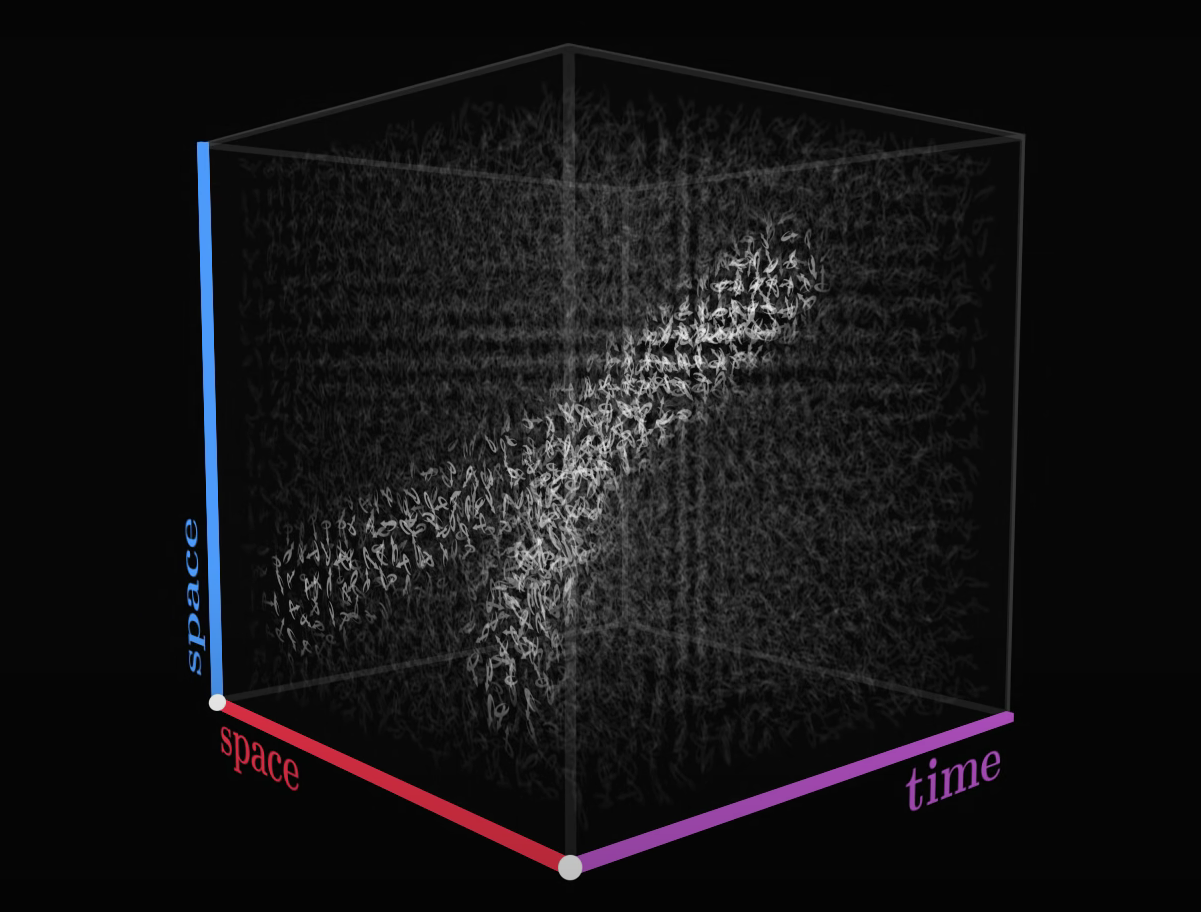
\includegraphics[width=0.7\textwidth]{qft.png}
          \caption{Illustration of a field}
      \end{figure}
\end{frame}


\begin{frame}{Correlation functions}
    In the operator formalism
    \begin{equation}
        \langle 0 | \mathcal{T}\left(\varphi(x) \phi(y)\dots\right) |0\rangle
    \end{equation}
    In the path-integral formalism
    \begin{equation}
        \frac{1}{Z}\int \mathcal{D}\psi ~ \varphi(x)\phi(y)\dots e^{i\mathcal{S}(\psi)}
    \end{equation}
    with $Z = \int \mathcal{D}\psi ~ e^{i\mathcal{S}(\psi)}$
\end{frame}


\subsection{2D CFTs}


\begin{frame}{Conformal field theories}\Large
    \begin{figure}
        \centering
        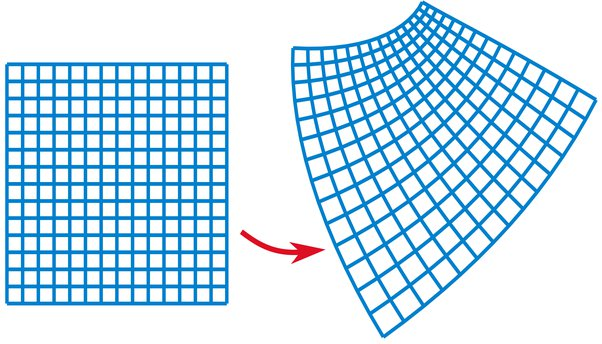
\includegraphics[width=0.65\textwidth]{conformal}
        \caption{Conformal Transformation}
    \end{figure}
    \begin{equation}
        \eta^{\mu\nu}\rightarrow \lambda(x^\alpha)\eta^{\mu\nu}
    \end{equation}
\end{frame}


\begin{frame}{Conformal generators}\Large
    \begin{equation}
        <M_{\mu\nu}, P_\mu, K_\mu, D>
    \end{equation}
    \begin{figure}
        \centering
        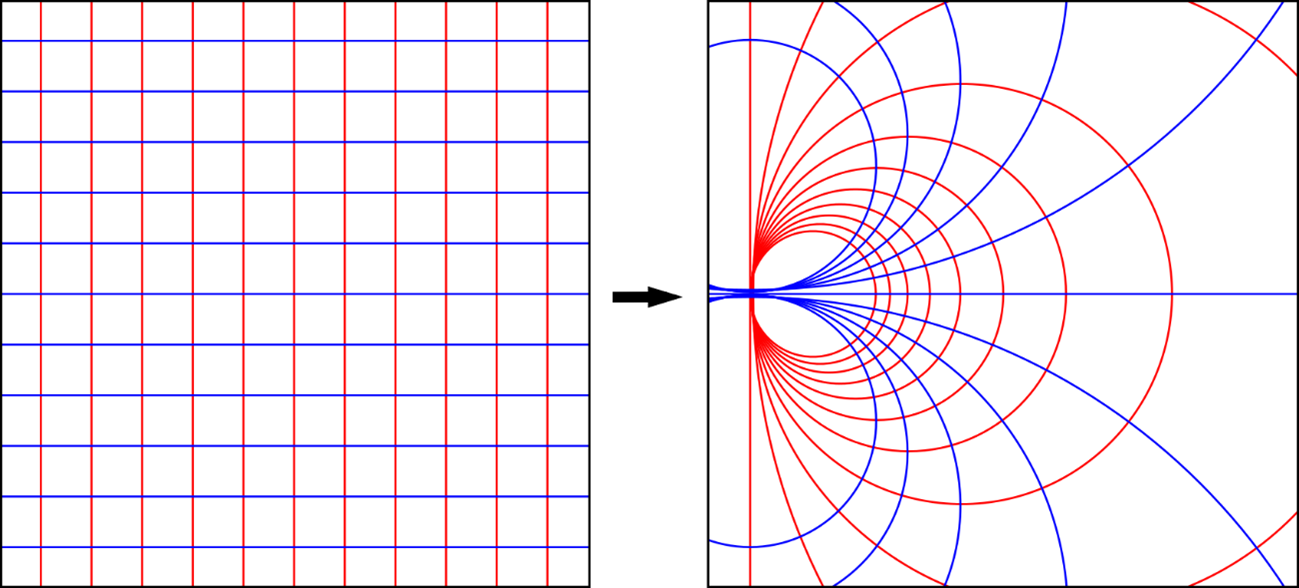
\includegraphics[width=0.65\textwidth]{specialconformal}
        \caption{Special Conformal Transformation}
    \end{figure}
\end{frame}


\begin{frame}{2D CFTs and chirality}
    \begin{alertblock}{Chiral coordinates}
        \begin{equation}
            z = x + t\qquad \bar{z} = x - t
        \end{equation}
    \end{alertblock}
    The energy-momentum tensor decouples
    \begin{equation}
        \begin{aligned}
            T^{z\bar{z}} = T^{\bar{z}z}& = 0 \\ T^{zz} = T(z) \qquad &T^{\bar{z}\bar{z}} = \bar{T}(\bar{z})
        \end{aligned}
    \end{equation}
\end{frame}

\begin{frame}{Virasoro algebra}
    \begin{equation}
        T(z) = \sum_n L_n z^{-n-2}
    \end{equation}
    \begin{alertblock}{The Virasoro algebra}
        \begin{equation}
            [L_m, L_n] = (m-n)L_{m+n} + \frac{c}{12}(m^3-m)\delta_{m+n, 0}
        \end{equation}
    \end{alertblock}
    Partition of the Hilbert space
    \begin{equation}
        \mathcal{H} = \sum_{i, j} V(c, h_i) \otimes \overline{V}(c, \bar{h}_j)
    \end{equation}
\end{frame}

\begin{frame}{RCFTs} \Huge
    \begin{equation}
        \mathcal{H} = \sum_{i, j} V_{\mathcal{A}}(h_i) \otimes \overline{V}_{\bar{\mathcal{A}}}(\bar{h}_j)
    \end{equation}
\end{frame}


\subsection{Mathematical aspects}


\begin{frame}{OPE and algebra}
    \begin{equation}
        A(z)B(w) \sim \sum_i \frac{1}{(z-w)^i} C_i(w)
    \end{equation}
    The structure is called a \alert{vertex algebra}
    \begin{alertblock}{$\mathcal{W}$-algebra}
        A $\mathcal{W}$-algebra is a chiral algebra of the form $<T, \varphi^{h_1}, \varphi^{h_2}, \dots >$, written $\mathcal{W}(2, h_1, h_2, \dots)$
    \end{alertblock}
\end{frame}



\section{The WZW model}
\subsection{The Sigma Model}


\begin{frame}{The Sigma model}
    Defined from $\Sigma$ to $X$ by the action 
    \begin{equation}
        \mathcal{S}(\varphi) = \frac{1}{2}\int_{\Sigma} g^{ij}(\varphi) \partial^\mu \varphi_i \partial_\mu \varphi_j
    \end{equation}
    \begin{itemize}
        \item $\mathcal{M} \rightarrow \mathbb{C}$ : non-interacting, massless quantum mechanics
        \item $\mathbb{R} \rightarrow \mathcal{M}$ : relativistic particle
        \item $\mathbb{R}^2 \rightarrow \mathcal{M}$ : string on a manifold
    \end{itemize}
\end{frame}

\begin{frame}{Sigma model on Lie algebras}
    \begin{figure}
        \centering
        \includegraphics[width=0.6\textwidth]{string_manifold}
        \caption{Illustration of a string on a Lie group}
    \end{figure}
    \begin{equation}
        \mathcal{L} = 2 \text{Tr}(g^{-1}\partial g ~ g^{-1}\overline{\partial} g)
    \end{equation}
\end{frame}

\begin{frame}{Two levels of conformality}
    \begin{figure}
        \centering
        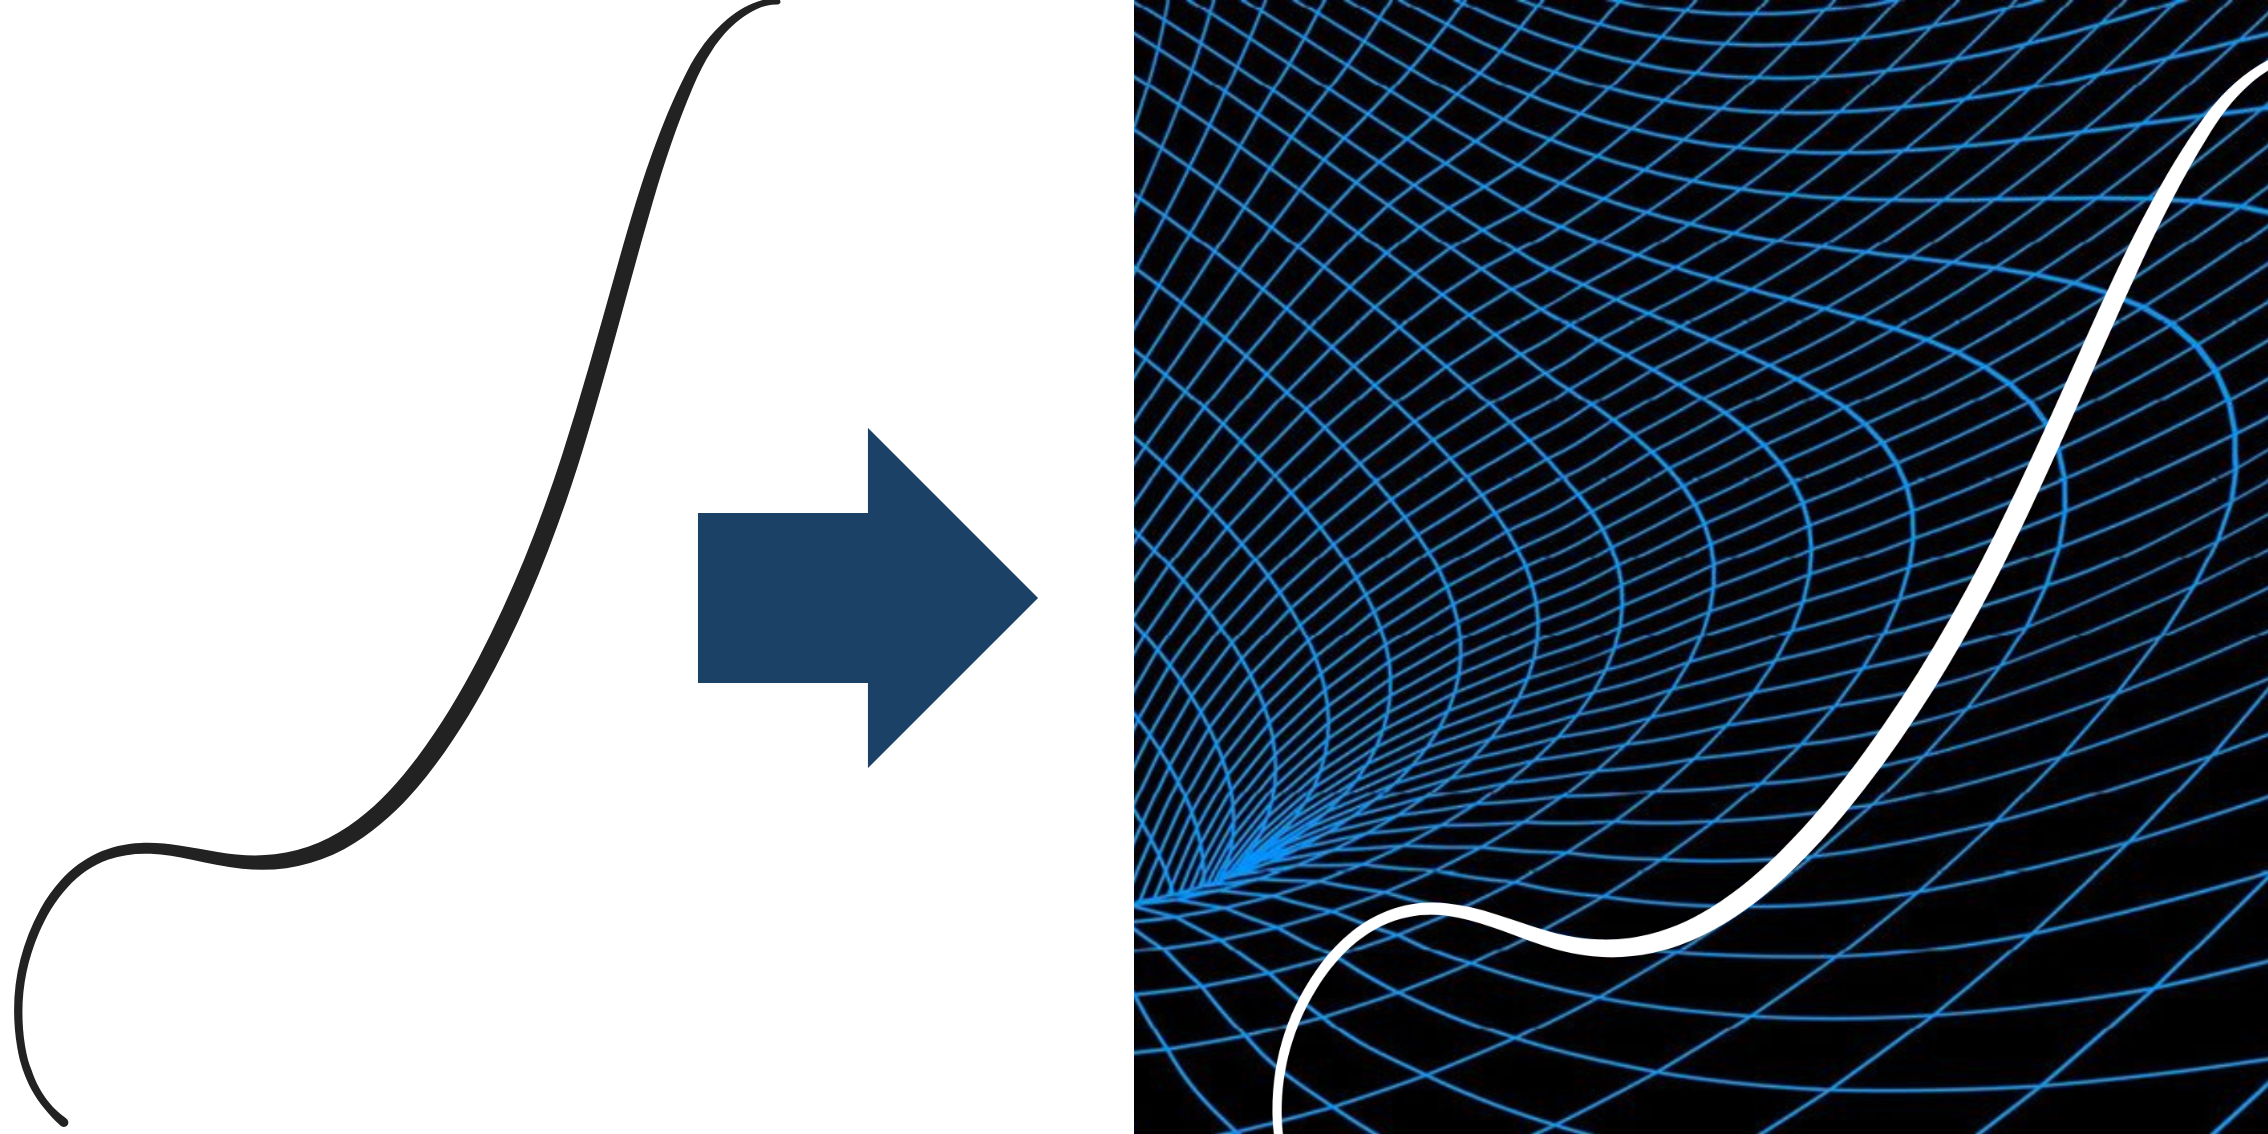
\includegraphics[width=0.7\textwidth]{string_field}
        \caption{Time slice of the base manifold and target manifold}
    \end{figure}
    \begin{alertblock}{$G\times G$ symmetry}
        \begin{equation}
            J^\mu = g^{-1}\partial^\mu g \qquad \tilde{J}^\mu = \partial^\mu g~g^{-1}
        \end{equation}
    \end{alertblock}
\end{frame}


\subsection{Adding the topological term}


\begin{frame}{Geometrical obstruction}\LARGE
    Equation of conservation:
    \begin{equation}
        \partial J^{\bar{z}} + \overline{\partial}J^z = 0
    \end{equation}
    But
    \alert{\begin{equation}
        \begin{aligned}
            \partial J^{\bar{z}} &= \overline{\partial}J^z = 0 \\
            & \Rightarrow [J^\mu, J^\nu] = 0
        \end{aligned}
    \end{equation}} 
\end{frame}

\begin{frame}{The topological term}
    \begin{figure}
        \centering
        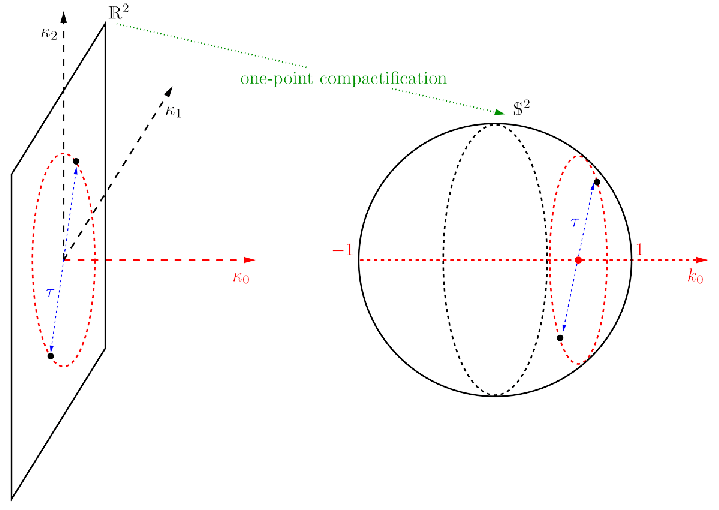
\includegraphics[width=0.4\textwidth]{compactification}
        \caption{Compactification of $\mathbb{R}^2$ into $\mathbb{S}^2$}
    \end{figure}
    \begin{equation}
        \mathcal{S}_{\text{W}} = \int_{\mathbb{B}^3}\text{Tr}(\wedge^3 g^{-1}\text{d} g)
    \end{equation}
\end{frame}

\begin{frame}{The WZW model}
    We consider $\frac{k}{2\pi}\mathcal{S}_{\text{W}}$, for $k\in \mathbb{Z}$ the \alert{level of the theory}. The equation of conservation becomes
    \begin{equation}
        \left(1 + \frac{k}{2\pi \lambda}\right) \partial J^{\bar{z}} + \left(1 - \frac{k}{2\pi \lambda}\right) \overline{\partial}J^z = 0
    \end{equation}
    So we consider
    \begin{equation}
        \mathcal{S}_{\text{WZW}} = \frac{k}{\pi}\int_{\mathbb{S}^2} \text{Tr}(g^{-1}\partial g~ g^{-1}\overline{\partial}g) - \frac{k}{2\pi}\int_{\mathbb{B}^3}\text{Tr}(\wedge^3 g^{-1}\text{d}g)
    \end{equation}
    With conserved currents
    \begin{equation}
        J(z) = \tilde{J}^z \qquad \bar{J}(\bar{z}) = J^{\bar{z}}
    \end{equation}
\end{frame}

\section{Reductions of the model}
\subsection{Reducing the model}


\begin{frame}{Toda field theory} \Large
    Study of $(\mathcal{A}, \overline{\mathcal{A}})$ such that 
    \begin{equation}
        \mathcal{A} = g\partial g^{-1} \qquad \overline{\mathcal{A}} = g\overline{\partial} g^{-1}
    \end{equation}
    \begin{equation}
        \partial \overline{\partial}g = \overline{\partial}\partial g
    \end{equation}
    \begin{equation}
        \mathcal{A} \in \mathfrak{g}_+\qquad \overline{\mathcal{A}} \in \mathfrak{g}_-
    \end{equation}

    We get the Casimir algebras
    \begin{equation}
        A_n \Rightarrow \mathcal{W}(2, 3, \dots n)
    \end{equation}
\end{frame}

\begin{frame}{Generalizing conditions} \LARGE
    We want to fix $J(z)$ along $\Gamma$
    \begin{equation}
        J(z) = M + j(z) \qquad j(z) \in \Gamma^{\perp}
    \end{equation}
    \begin{equation}
        \phi_\gamma(z) = \langle \gamma, J(z) \rangle - \langle \gamma, M \rangle = 0 \quad \forall \gamma \in \Gamma
    \end{equation}
\end{frame}

\subsection{Conditions}


\begin{frame}{First-classness of the conditions} \LARGE
    \begin{equation}
        \begin{aligned}
            \{\phi_\alpha, \phi_\beta&\} = 0 \\
            &\Rightarrow [\Gamma, \Gamma^\perp] \\
            &\Rightarrow [M, \Gamma] \subset \Gamma^\perp \\
            &\Rightarrow \Gamma \subset \Gamma^\perp 
        \end{aligned}
    \end{equation}
    which in particular implies
    \begin{equation}
        M \in [\Gamma, \Gamma]^\perp / \Gamma^\perp
    \end{equation}
\end{frame}

\begin{frame}{Conformality of the reduction}
    \begin{figure}
        \centering
        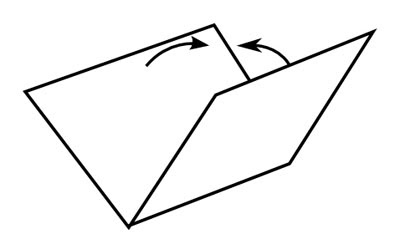
\includegraphics[width=0.3\textwidth]{valleyfold}
        \caption{Illustration of a valley fold}
    \end{figure}
    \begin{alertblock}{Gravity potential} 
        \begin{equation}
            E_p = \langle m\vec{g}, \vec{z} \rangle
        \end{equation}
    \end{alertblock}
    \begin{alertblock}{Our potential}
        \begin{equation}
            E_p = \langle J'(z), H\rangle
        \end{equation}
    \end{alertblock}
\end{frame}


\begin{frame}{Conditions on $H$} \huge
    \begin{equation}
        \begin{aligned}
            &H \in \Gamma^\perp \\
            &[H, \Gamma^\perp] \subset \Gamma^\perp\\ 
            &([H, M] + M) \in \Gamma^\perp
        \end{aligned}
    \end{equation}
    This makes us want to have 
    \begin{equation}
        [H, M] = -M
    \end{equation}
\end{frame}

\begin{frame}{The Drinfield-Sokolov gauge} \Large
    To compute the algebra, we should fix a gauge
    \begin{equation}
        J_{\text{red}}(z) = M + j_{\text{red}} \qquad j_{\text{red}} \in \mathcal{V}
    \end{equation}
    with 
    \begin{equation}
        \Gamma^\perp = [M, \Gamma] + \mathcal{V}
    \end{equation}
    we choose
    \begin{equation}
        \mathcal{V} = \Gamma^{\perp_\omega} \cap \Gamma^\perp \qquad \omega_M(\alpha, \beta) = \langle M, [\alpha, \beta]\rangle
    \end{equation}
\end{frame}

\begin{frame}{Last conditions} \huge
    For $\Gamma^{\perp_\omega}$ to exist
    \begin{equation}
        \Gamma \cap \text{Ker}(\text{ad}_M)
    \end{equation}
    For positive conformal dimensions
    \begin{equation}
        \Gamma ^\perp \subset \mathfrak{g}_{>-1}
    \end{equation}
\end{frame}

\subsection{The algebra $\mathcal{W}^k(\mathfrak{g}, x, f)$}


\begin{frame}{Good gradings} \LARGE
    \begin{alertblock}{Good Grading}
        $(H, M)$ such that $H$ is diagonalizable, $M \in \mathfrak{g}_{-1}$ and 
        \begin{equation}
            \mathfrak{g}^M \subset \mathfrak{g}_{\leq}
        \end{equation}
    \end{alertblock}
    We write $\mathcal{W}^k(\mathfrak{g}, x, f)$
\end{frame}

\section{Classifying through pyramids}
\subsection{Good gradings}


\begin{frame}{Good gradings}
    A pair $(x, e)$ such that $x$ induces a grading and
    \begin{itemize}
        \item $\text{ad}_e$ is injective starting from $\mathfrak{g}_{<}$
        \item $\text{ad}_e$ is surjective arriving in $\mathfrak{g}_{>}$
    \end{itemize}

    \begin{figure}
        \centering
        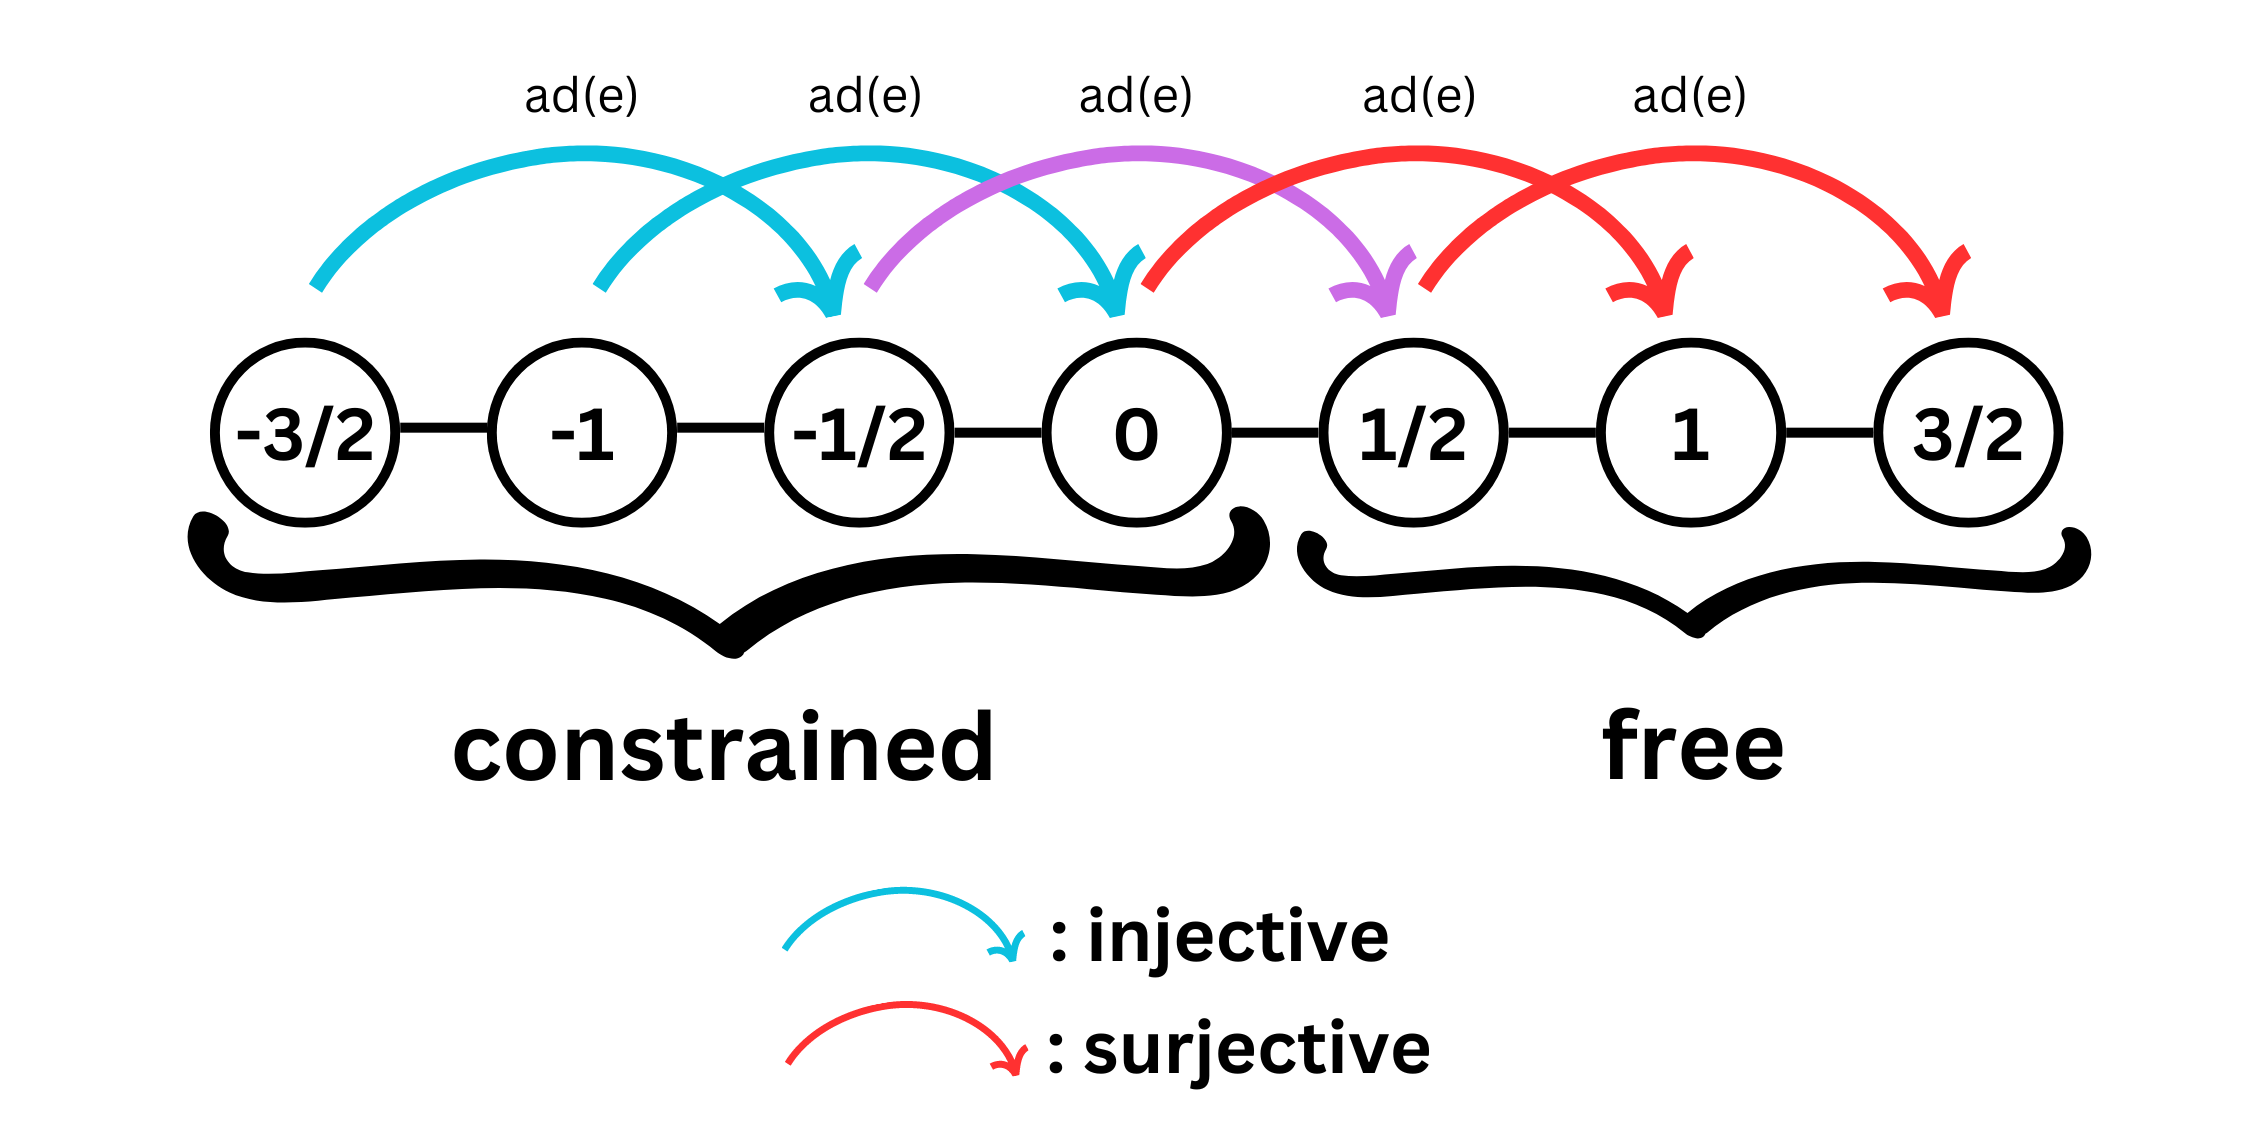
\includegraphics[width=0.7\textwidth]{goodgrading}
        \caption{Illustration of a good grading}
    \end{figure}
\end{frame}


\subsection{Pyramids}


\begin{frame}{From shifting constant to blocks}
    \begin{figure}
        \centering
        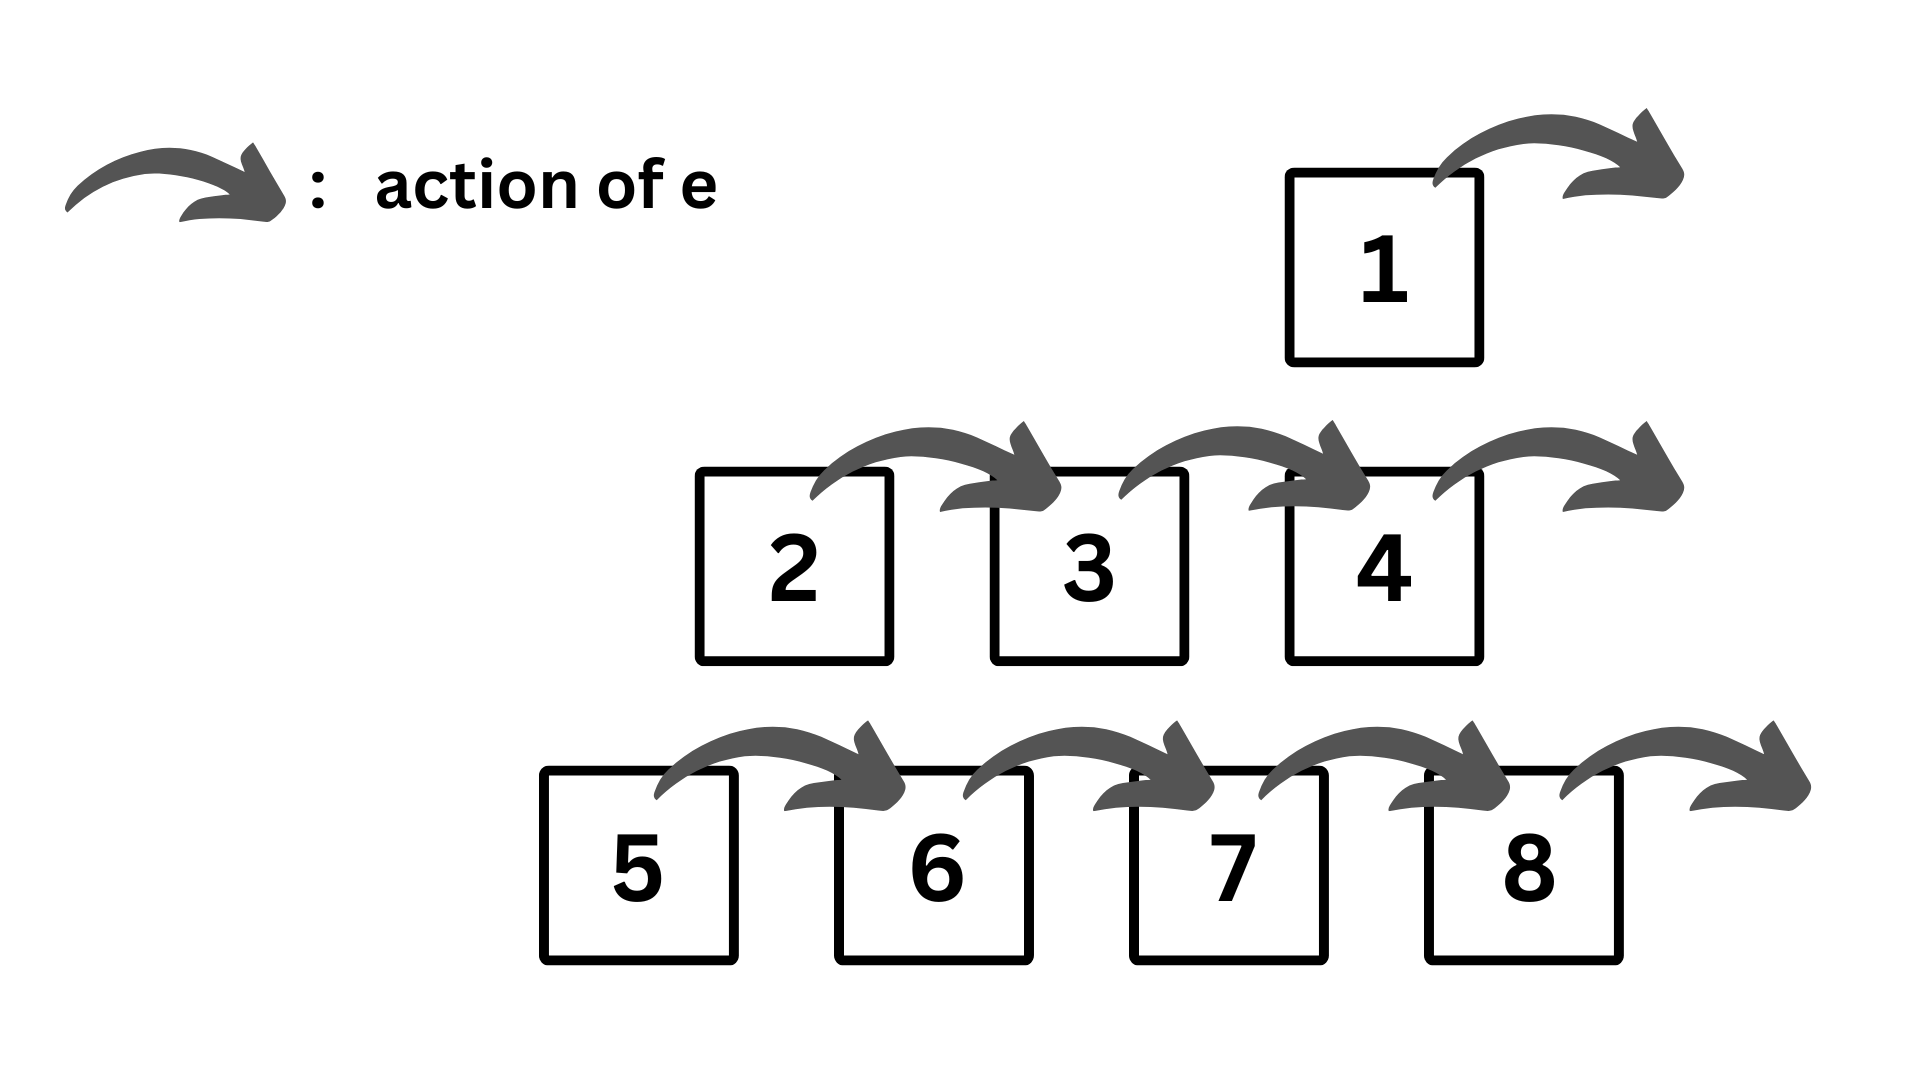
\includegraphics[width=0.9\textwidth]{pyramid}
        \caption{Representation of the nilpotent element $e$ in a pyramid}
    \end{figure}
\end{frame}

\begin{frame}{From Hamiltonian term to pyramids}
    \begin{figure}
        \centering
        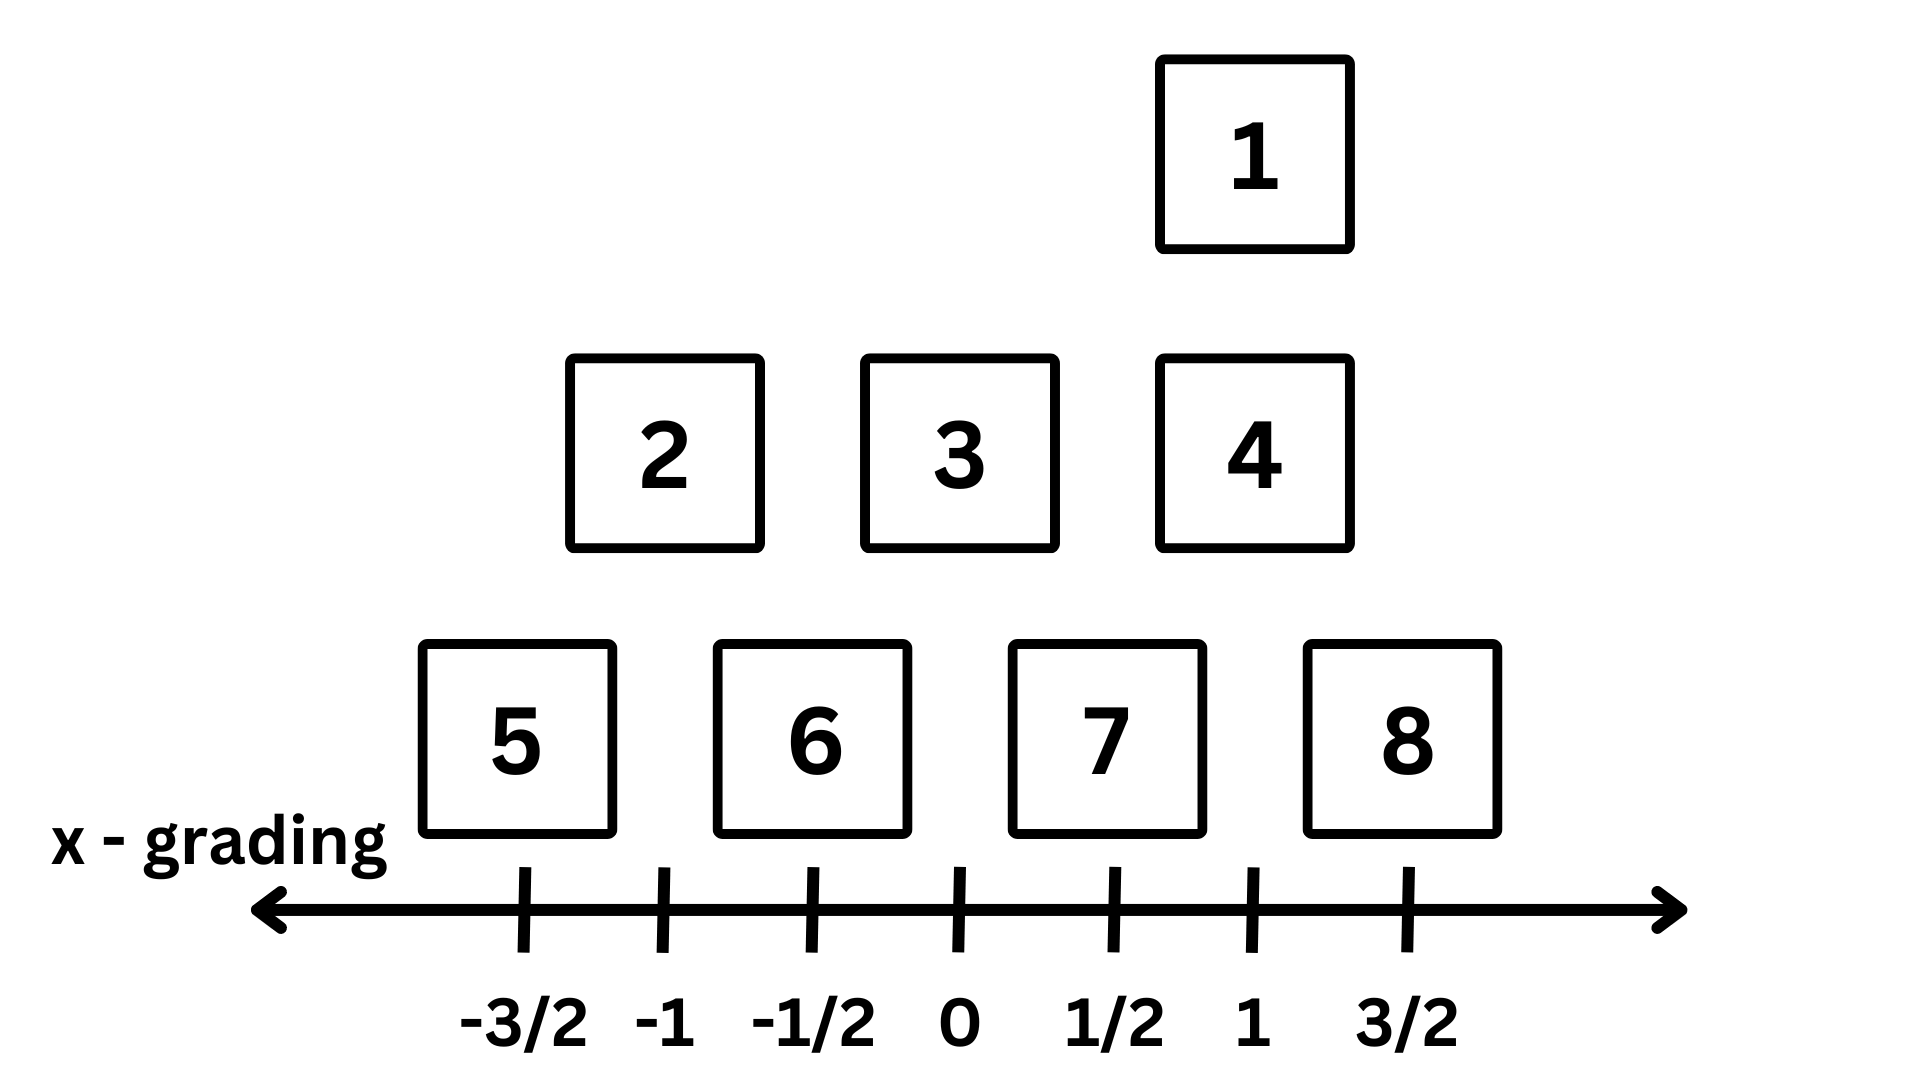
\includegraphics[width=0.9\textwidth]{pyramid2}
        \caption{Representation of the diagonalizable element $x$ in a pyramid}
    \end{figure}
\end{frame}

\begin{frame}{Reading pyramids}
    \begin{figure}
        \centering
        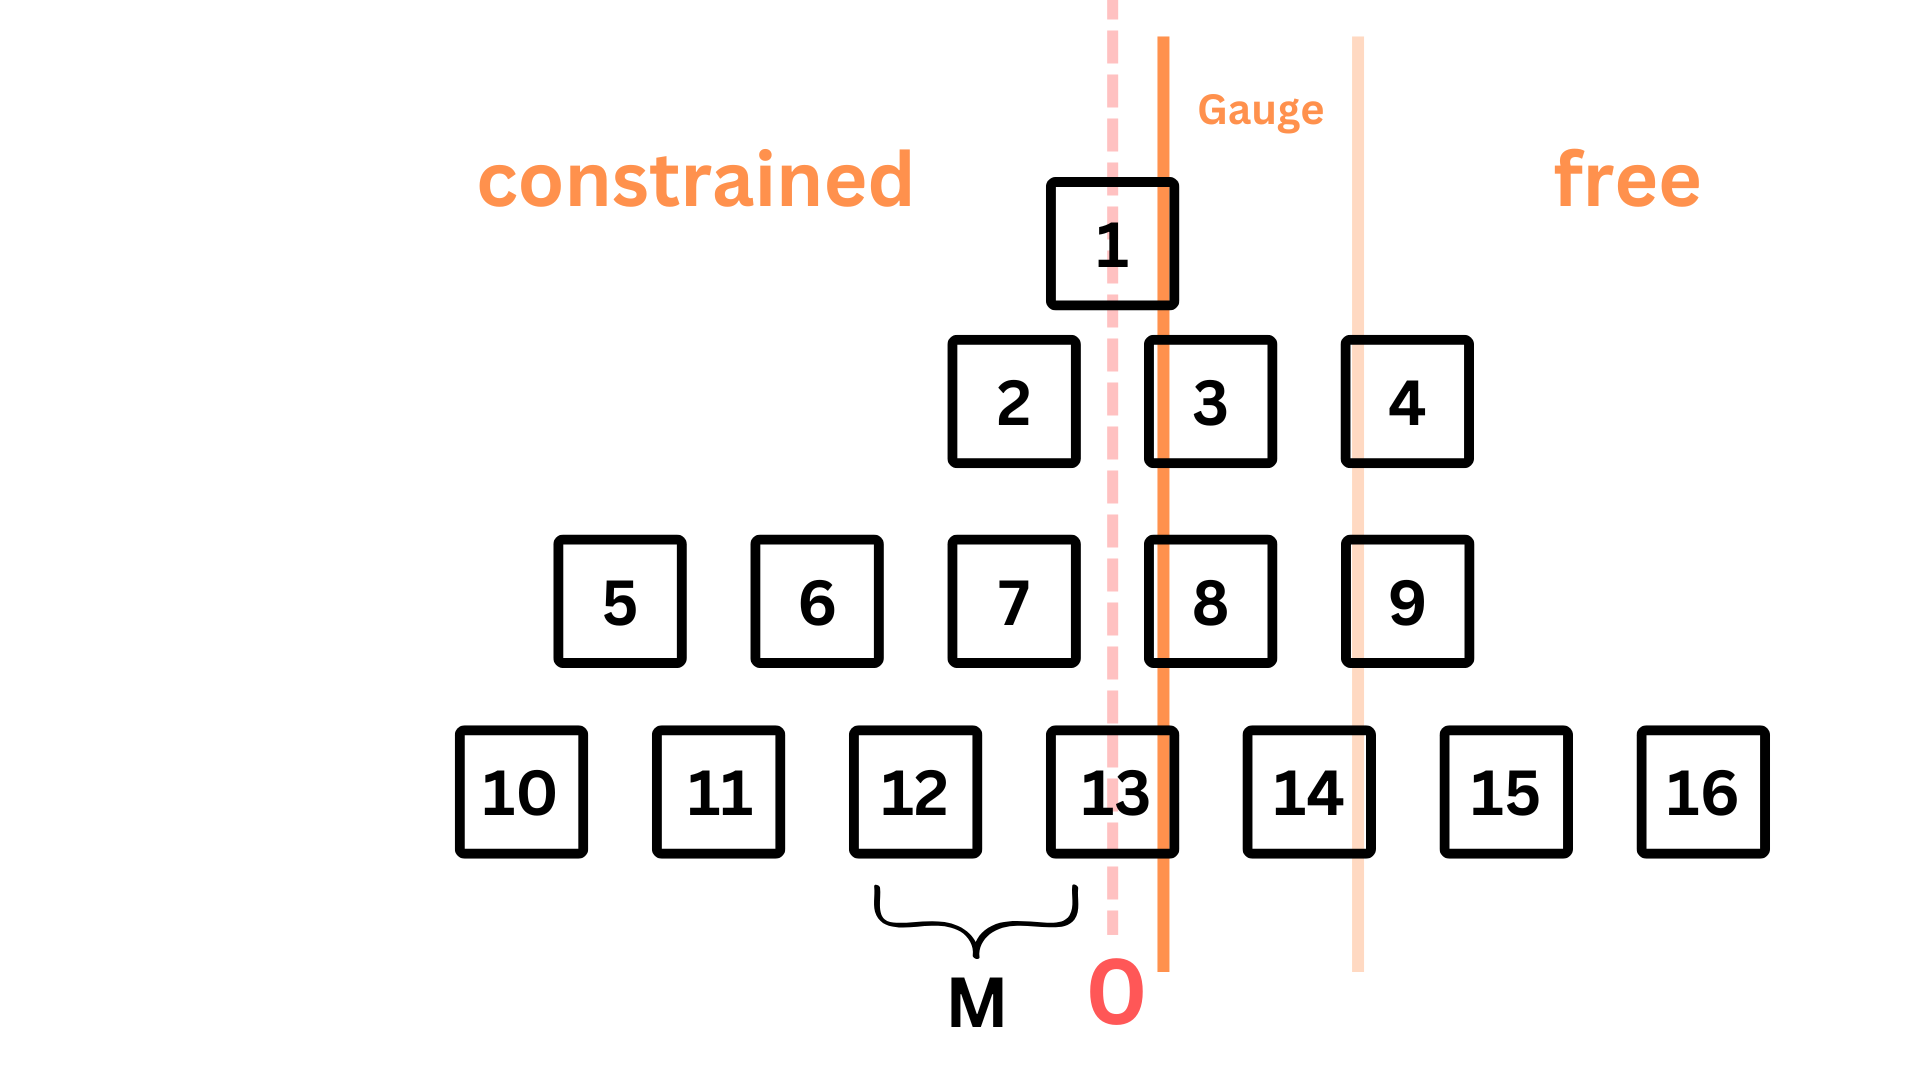
\includegraphics[width=0.9\textwidth]{readingpyramids}
        \caption{Diagram of the informations in a pyramid}
    \end{figure}
\end{frame}


\end{document}